\subsection{Segmentation 3D}
%recuperation d'un objet dans l'environnemnt -> interaction utilisateur
%dire que la création d'une base de connaissance est plus utile que pour le corps humain
La première étape lors de ce projet va être de segmenter les images que nous recevons de 
la caméra. Les informations contenues dans une image 3D sont nombreuses et nous devons
déterminer les éléments importants pour nos traitements. Dans notre scène,
nous avons besoin des objets proches ou du corps de la personne en face de la caméra, mais 
l'environnement autour des ces objets clés n'est pas important et doit être supprimé pour
gagner du temps lors de nos traitements.
Une seconde segmentation est nécessaire pour le traitement du corps humain. Pour cette étape du projet,
nous devons segmenter le corps en plusieurs parties pour pouvoir, par la suite, les reconnaitre. Si cette
seconde segmentation n'est pas réalisée, il ne nous sera pas possible de reconnaître les mains ou encore
la tête si nous ne savons pas délimiter les parties du corps.  

\begin{figure}[!ht]
  \begin{center}
    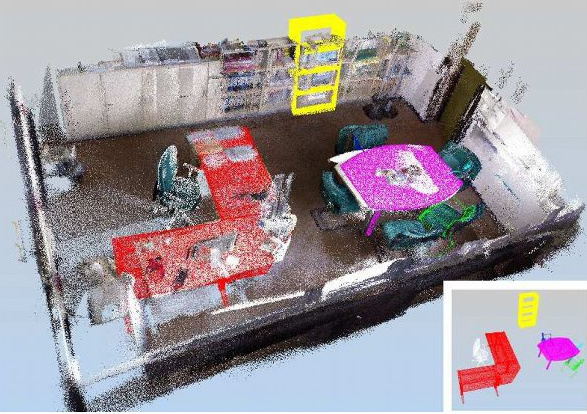
\includegraphics[width=8cm]{image/segmentation.png}
    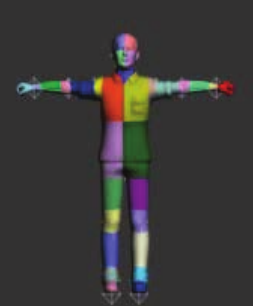
\includegraphics[width=5cm]{image/bodySegmentation.png}
    \caption[The LOF caption]{Résultat attendu pour la segmentation d'un environnement intérieur\footnotemark et du corps humain}
  \end{center}
\end{figure}
\footnotetext{source : \url{http://kos.informatik.uni-osnabrueck.de/icar2013/}}
 
\subsubsection{Segmentation d'un environnement intérieur}
De nombreux travaux ont été réalisés dans la segmentation d'image 2D avant que les caméras 3D ne soient
ouvertes au grand public. Les premières méthodes de segmentation reposaient sur la détection de contour
comme pour la méthode de P. Arbelaez et al\cite{2DSegmentation1}. Leur méthode repose sur le détecteur
de contour gPb qui est composé d'un seuillage sur la luminance et sur la couleur, et d'une détection
de texture. La fermeture des contours se fait ensuite en utilisant les superpixels. D'autres méthodes
2D utilisent un simple seuillage en utilisant par exemple la méthode de N. Otsu\cite{Otsu} pour binariser
l'image et ainsi la segmenter.\\

%peut etre que l on peut rajouter des publi utilisant la depthmap
%voir si on sépare la depthmap et le nuage de point
Avec l'arrivée des caméras 3D, de nombreuses recherches ont été effectuées sur la segmentation d'image à partir
des informations extraites de ce type de caméra. S.A.A Shah et al\cite{3DSegmentation1} utilisent les informations
de l'image de profondeur afin de calculer un vecteur sur chaque pixel. Ce vecteur s'obtient en calculant la divergence 
entre les pixels. En applicant un seuillage sur les vecteurs, ils obtiennent une segmentation de l'environnement 
qui leur permet de détecter des objets dans une pièce. Cette méthode est efficace lorsque l'objet que l'on 
cherche à détecter est proche de la caméra. Il est possible à partir de l'image de profondeur, de créer un 
nuage de points, ce qui permet d'obtenir les coordonnées 3D des points présents dans l'image de profondeur. Les informations 
qu'il est possible d'extraire d'un nuage de points sont différentes, et des méthodes de segmentation se sont développées autour de ces informations.\\

T. Rabbani et al\cite{pointCloudSegmentation} utilisent les informations obtenues dans un nuage de points afin 
de calculer les normales de chaque point. Ils segmentent ensuite l'image en comparant les normales et en appliquant
un seuillage sur cette comparaison. Si les angles formés par les normales du point courant et de ces voisins sont inférieurs au seuil alors
les points appartiennent à la même région.\\
 
Nous pouvons voir que les méthodes citées précédemment sont efficace pour segmenter une scène comportant des objets,
mais elles ne sont pas applicables à un corps humain. Le principal défaut de ces méthodes pour le corps humain est 
que celui-ci est trop lisse. La différence entre les normales ou entre les vecteurs de pixel n'est pas assez important
et celle-ci est trop instable pour que cela s'adapte sur le corps humain qui peut adopter de nombreuses postures.

\subsubsection{Segmentation des parties du corps humain}
La segmentation du corps humain est un sujet très complexe, car contrairement aux objets, celui-ci bouge et adopte
des postures différentes. La méthode la plus souvent utilisée pour résoudre cette problématique est de déterminer
la posture de l'utilisateur, puis de cette posture, déterminer les différentes partie du corps à partir de la labellisation
qui doit être réalisée sur la base de connaissance. 
Ces méthodes nécessitent d'avoir une base de connaissance contenant de nombreuses postures qui doivent
être segmentées et labelisées avec les différentes parties du corps. J. Shotton et al\cite{kinectSegmentation} ont
créé une base d'apprentissage en calculant un descripteur
et ils utilisent une technique d'apprentissage automatique appelée forêt d'arbres décisionnels\cite{randomDecisionForest}. 
Le descripteur de J. Shotton et al\cite{kinectSegmentation} utilise les informations de l'image de 
profondeur pour déterminer quelle posture a l'utilisateur. Ils utilisent une caractèristique reposant sur la valeur
de deux pixels, un pixel x et un pixel dont l'offset par rapport au pixel x a été défini.
Lorsque l'utilisateur bouge, le descripteur utilisé précédemment est recalculé sur l'image courante et le résultat 
est comparé au posture de la base d'apprentissage.\\

\begin{figure}[!ht]
  \begin{center}
    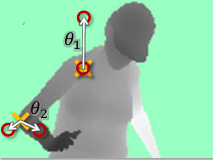
\includegraphics[width=6cm]{image/shotton.png}
    \caption{Deux exemples de caractèristique du descripteur de J. Shotton et al\cite{kinectSegmentation}. 
    La croix jaune correspond au pixel à classifier et le cercle rouge correspond au pixel décalé.}
  \end{center}
\end{figure}

La méthode de J. Shotton et al\cite{kinectSegmentation} est efficace pour de nombreuses parties du corps, 
mais reste instable sur les parties de la main comme le poignet et son centre. Mais cette méthode permet 
tout de même de déterminer approximativement les parties du corps occultées.\\

Comme pour la méthode précédente B. Yoo et al\cite{RDB} utilisent les images de profondeur pour déterminer
la posture de l'utilisateur. Cependant, leur descripteur repose sur des caractèristiques plus complexes comme
l'élongation 3D de la forme du corps, le centre de gravité, la rectangularité de la forme ou encore la 
dissymétrie. Grâce à ces caractèristiques, ils forment un descripteur qu'il passe dans leur propre outil
d'apprentissage automatique appelé \og Randomized Decision Bush \fg.\\

Y. Liu et al\cite{GIF} ont développé un autre descripteur spécifique à la reconnaissance de la posture du corps
humain appelé \og Geodesic Invariant Feature \fg(GIF). 
Ce descripteur se base sur le calcul de la distance géodésique. La distance géodésique est la distance
entre deux points d'un modèle 3D en ne passant que par les arrêtes de ce modèle. Etant donné que ce n'est pas un
modèle 3D que fournit la Kinect, mais un nuage de points, les auteurs forment un maillage en créant \textit{n} arrêtes avec
les \textit{n} points les plus proches pour un point donné. Cette distance géodésique permet de connaitre l'orientation
des points. Cette orientation est appliquée sur d'autres caratéristiques sensibles à la rotation, ce qui permet
à ces caractéristiques d'être invariantes en rotation. 

\begin{figure}[!ht]
  \begin{center}
    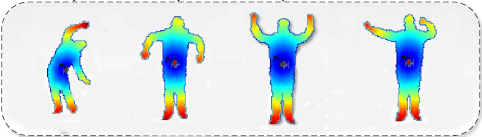
\includegraphics[width=12cm]{image/geodesic.png}
    \caption{Distance géodésique d'un corps humain}
  \end{center}
\end{figure}

%TODO voir si on ajoute la partie avec pca
\subsection{Reconnaissance d'objets}
La reconnaissance d'objets est un sujet assez vaste dans le monde de l'imagerie et il existe de nombreuses
méthodes dans le domaine, que ce soit pour des images 2D ou 3D. Dans le cas d'image 3D, l'approche de reconnaissance
d'objet commence par le calcul de descripteur, ce qui correspond à un ensemble de caractèristiques représentant un objet spécifique. 
Ce descripteur va ensuite être utilisé dans un classifieur afin de réaliser une base comportant les caractèristiques de 
l'ensemble des objets que nous souhaitons reconnaître par la suite.
%la méthode la plus utilisée
%est le calcul de descripteur, ce qui correspond à un ensemble de caractèristiques représentant un objet spécifique.

\subsubsection{Calcul de descripteur}
\label{descriptor}
Le nombre de descripteurs qui existent dans le domaine de l'image 3D est assez important, c'est pourquoi pour ce rapport,
nous allons nous contenter de décrire seulement les plus utilisés. Le descripteur D2\cite{D2} est un des outils de 
comparaison de forme 3D les plus simple à réaliser. Il se repose sur le calcul de la distance euclidienne entre 
chaque point du modèle 3D. L'ensemble de ces distances permet de créer un histogramme 1D et de comparer ces histogrammes
afin de reconnaître un objet. Ce descripteur fournit de bons résultats lorsque les objets à reconnaître sont très 
différents.\\

Le descripteur PFH\cite{PFH} (Point Feature Histograms) est un outil permettant de calculer la courbure moyenne d'un voisinage de points en utilisant un histogramme multi-dimensionnel. Le calcul de la courbure et le fait que ce soit une généralisation permettent d'être invariant 
en translation, en rotation et en densité de points, et permet également d'être moins sensible au bruit présent dans le nuage de points. Le voisinage 
dépend de la distance des points avec le point central et il ne peut excéder un certain nombre de voisin s
(voir Fig. \ref{fig:pfhNeighborhood}).\\

\begin{figure}[!ht]
  \begin{center}
    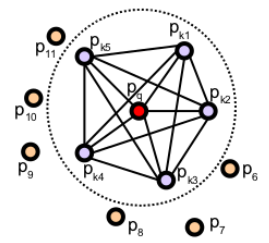
\includegraphics[width=6cm]{image/PFH.png}
    \caption{Exemple de voisinage pris en compte dans le calcul de la courbure du descripteur PFH}
    \label{fig:pfhNeighborhood}
  \end{center}
\end{figure}

Le descripteur PFH calculé en un point correspond à la relation que ce point a avec l'ensemble des points de son voisinage. Cette relation
est la différence des normales entre deux points. Chaque classe de l'histogramme est composée de l'ensemble des points du voisinage dont 
la relation avec le point central est similaire. Une version améliorée du descripteur a été proposée par R. B. Rusu et al\cite{FPFH} appelé
FPFH (Fast Point Feature Histograms). Cette version est plus rapide, car elle calcule un descripteur PFH simplifié, puis elle construit
de nouveaux histogrammes à partir des histogrammes simplifiés précédents (voir Fig. \ref{fig:fpfhNeighborhood}).\\

\begin{figure}[!ht]
  \begin{center}
    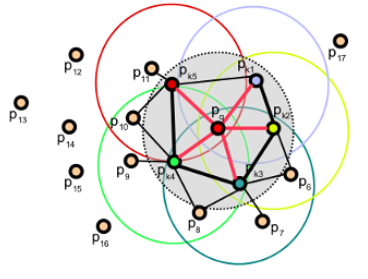
\includegraphics[width=7cm]{image/FPFH.png}
    \caption{Exemple de voisinage pris en compte dans le calcul de la courbure du descripteur FPFH}
    \label{fig:fpfhNeighborhood}
  \end{center}
\end{figure}

D. G. Lowe\cite{SIFT} a créé un descripteur appelé \og scale-invariant feature transform \fg(SIFT) qui crée
des points clés dans une image 2D et calcule des descripteurs sur ces points. Ce descripteur permet entre autre
de détecter des points clés similaires dans deux images différentes d'une même scène, tant que les angles de vue
sont suffisamment petits. Les points clés de ce descripteur sont des zones circulaires positionnées sur les extremas 
dans l'espace des échelles, le facteur d'échelle étant proportionnel à la taille de la zone d'intérêt. Une fois que
que l'on a trouvé la position des points clés, il faut déterminer leur orientation en calculant le gradient dans le voisinage
du point clé. Grâce aux orientations des voisins des points clés, il est possible de créer un histogramme des orientations. Ainsi
l'orientation du point clé correspond aux pics les plus importants de l'histogramme.
La construction de ces points clés permet à ceux-ci d'être invariants aux changements d'échelle et aux rotations.

%TODO SHOT -> voir si on en parle
\subsubsection{Apprentissage automatique}
L'apprentissage automatique est un outil permettant à une machine de prendre des décisions rapidement.
Pour fonctionner, cet outil a besoin de données déjà traitées sur un domaine précis. Il existe de nombreuses
techniques d'apprentissage automatique. Lors de ce projet, je me suis intéressé à deux techniques en 
particulier qui sont parmi les plus utilisées dans le domaine de l'image : la \og forêt d'arbres décisionnels \fg \ et les
\og machines à vecteurs de support \fg (SVM).\\

Le principe de la forêt d'arbres décisionnels\cite{randomDecisionForest} est de créer un ensemble d'arbres.
Dans le cas de la méthode de J. Shotton et al\cite{kinectSegmentation}, chaque arbre correspond à une posture.
Les noeuds des arbres correspondent aux caractéristiques calculées. L'algorithme teste des noeuds lui permettant ainsi de tracer un
chemin vers une feuille qui donne un résultat. L'arbre dont la feuille nous donne le résultat le plus proche 
de la valeur recherchée nous fournit la solution à notre problème.\\

\begin{figure}[!ht]
  \begin{center}
    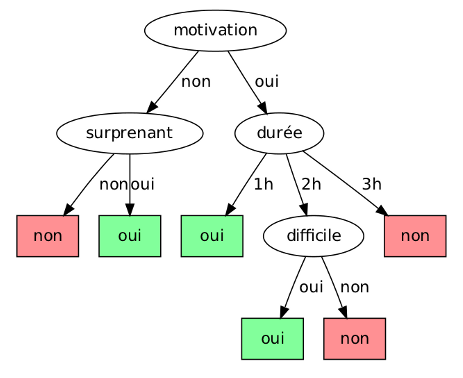
\includegraphics[width=7cm]{image/randomForest.png}
    \caption[The LOF caption]{Exemple d'arbre de décision\footnotemark }
  \end{center}
\end{figure}
\footnotetext{source : \url{https://scaron.info/doc/intro-arbres-decision/}}

Les machines à vecteurs de support\cite{SVM}, quant à eux, sont une classe d'algorithmes d'apprentissages supervisés permettant la
résolution de 
problèmes de discrimination non linéaire. Le principe des SVM est d'apprendre un séparateur dans le but de classifier les données à partir
d'une base d'apprentissage. Dans le cas d'un problème linéaire, les SVM recherchent l'hyperplan le plus approprié à la séparation des données
dans l'espace vectoriel, en minimisant les pertes de points dans la base d'apprentissage. Lorsque le problème est non linéaire,
les SVM changent l'espace dans lequel les points sont projetés à l'aide d'une fonction noyau.

\subsubsection{L'approche sac de mots (bag of word)}
Le sac de mots est une représentation dont la première utilisation était de décrire un document texte en fonction d'un dictionnaire.
Le dictionnaire est un ensemble de mots capable de décrire tous les textes.
Le principe est de compter le nombre d'occurence d'un mot dans un texte, et ce pour chaque mot du dictionnaire. Cette représentation
a ensuite été utilisée dans le domaine de la vision par ordinateur appelé \og bag of visual world \fg\cite{BagOfWord} 
en remplaçant le dictionnaire de mot par un dictionnaire
de caractèristiques. Grâce à cette représentation, nous obtenons un vecteur de la taille du dictionnaire, composé du nombre 
d'occurence de chaque caractèristique. L'intérêt de cette représentation est d'uniformiser la structure des données
afin d'avoir un vecteur de même taille pour toutes les images, mais cela nécessite une première phase de création du dictionnaire
avec l'ensemble des caractèristiques des images traitées. Nous obtenons ainsi un nouveau descripteur sous la forme d'un
histogramme dont ça taille est égale au nombre de caractèristique différente de chaque classe.

\begin{figure}[!ht]
  \begin{center}
    \includegraphics[width=8cm]{image/bagofwords.png}
    \caption[The LOF caption]{Schéma du fonctionnement de l'algorithme du bag of visual words\footnotemark }
  \end{center}
\end{figure}
\footnotetext{source : \url{http://www.ifp.illinois.edu/~yuhuang/sceneclassification.html}}

\subsection{Positionnement de modèle}
Afin de réaliser la correspondance entre deux modèles P. J. Besl et al\cite{ICP} développe l'algorithme \og iterative closest point \fg (ICP).
Cet algorithme recherche l'ensemble des translations et rotations nécessaires à la mise en correspondance de deux modèles similaires. Pour cela,
celui-ci fonctionne en quatre étapes :
\begin{itemize}
  \item Associer les points grâce aux critères du plus proche voisin. Pour cela, il suffit de calculer la distance euclidienne d'un
   point avec tous les autres points qui font partis du balayage que nous voulons comparer et de prendre la distance la plus petite.
  \item Estimer la transformation des points grâce à une fonction d'erreur quadratique moyenne, permettant ainsi de trouver la meilleure
  transformation possible.
  \item Effectuer la transformation du nuage de points ayant la plus petite erreur.
  \item Itérer jusqu'à ce qu'on ait atteint la condition de fin fixée par l'utilisateur.
\end{itemize}
\ \\
Dans la bibliothèque PCL\cite{PCL}, S. Ushakov implémente une classe basée sur le moment d'inertie\footnote{\url{http://pointclouds.org/documentation/tutorials/moment\_of\_inertia.php\#moment-of-inertia}}
permettant de déterminer les axes principaux d'un nuage de points. Pour cela, cette classe calcule la matrice de covariance du nuage de points et 
en extrait les vecteurs propres. Le plus grand vecteur propre est considéré comme étant l'axe X et le plus petit devient l'axe Z, ce qui permet 
d'obtenir un système de coordonnées dans un référentiel local à l'objet.\\   
\begin{figure}[!ht]
  \begin{center}
    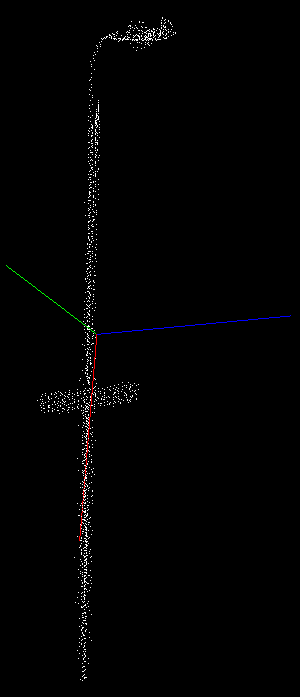
\includegraphics[angle=90,origin=c,width=8cm]{image/objectAxis.png}
    \caption{Résultat du calcul des axes sur un nuage de points grâce à la méthode utilisant le moment d'inertie}
  \end{center}
\end{figure}

\subsection{Interaction utilisateur}
T. Shao et al\cite{interactiveSeg} proposent, en plus d'avoir une méthode de segmentation automatique, d'améliorer leur 
segmentation en impliquant l'utilisateur dans le processus. Ainsi lorsque la segmentation d'une pièce comporte des erreurs, 
l'utilisateur est amené à rectifier les erreurs de la machine au travers d'une interface.
Pour cela les auteurs proposent à l'utilisateur de dessiner sur l'objet dont le label est erroné avec la couleur du label 
qui correspond, ainsi l'application change la couleur et le label de l'objet sélectionné.\\ 

\begin{figure}[!ht]
  \begin{center}
    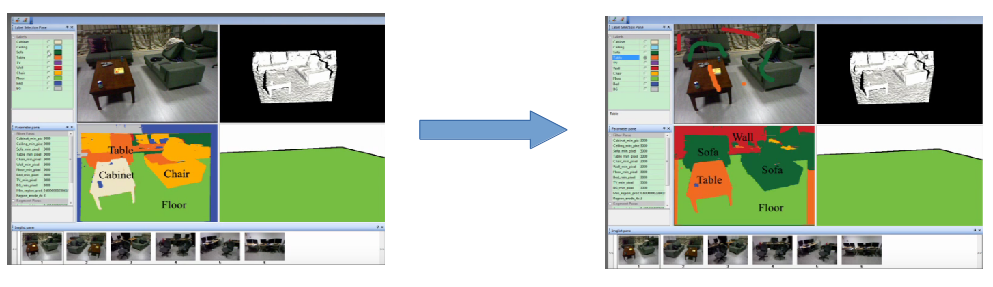
\includegraphics[width=16cm]{image/recoInteractive1.png}
    \caption{Résultat de la reconnaissance interactive de T. Shao et al\cite{interactiveSeg}}
  \end{center}
\end{figure}

Sur le même principe, J. Xiao et al\cite{interactionSeg2}
ont créé un système d'interaction afin de faciliter la création de leur base d'apprentissage. Pour cela, lorsque l'utilisateur 
clique sur l'image, il place un marqueur. Cela permet, en plaçant plusieurs marqueurs, de délimiter un objet. Lorsque le premier
marqueur a la même position que le dernier, le contour est terminé, et l'utilisateur est invité à donner un label à l'objet
qu'il vient de délimiter.

\begin{figure}[!ht]
  \begin{center}
    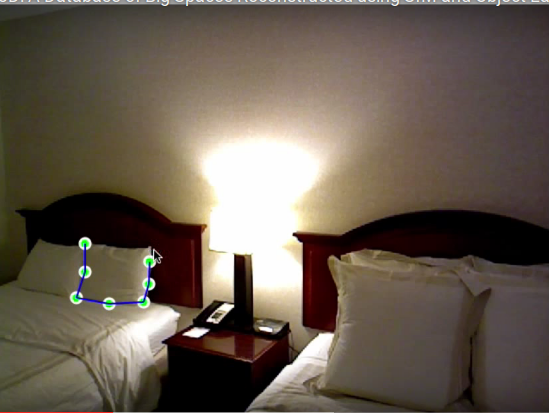
\includegraphics[width=7cm]{image/segInteractive1.png}
    \caption{Résultat de la sélection interactive de J. Xiao et al\cite{interactionSeg2}}
  \end{center}
\end{figure}
